% !TEX TS-program = pdflatex
% !TEX encoding = UTF-8 Unicode
\documentclass[border=0mm]{standalone}
% packages
\usepackage{tikz}
\usetikzlibrary{patterns}
\usepackage{amsmath,amssymb}
\usepackage{bm}
\usepackage{pgfplots}
\pgfplotsset{compat=1.15}
% start document
\begin{document}
% generated by ROOT (CERN)
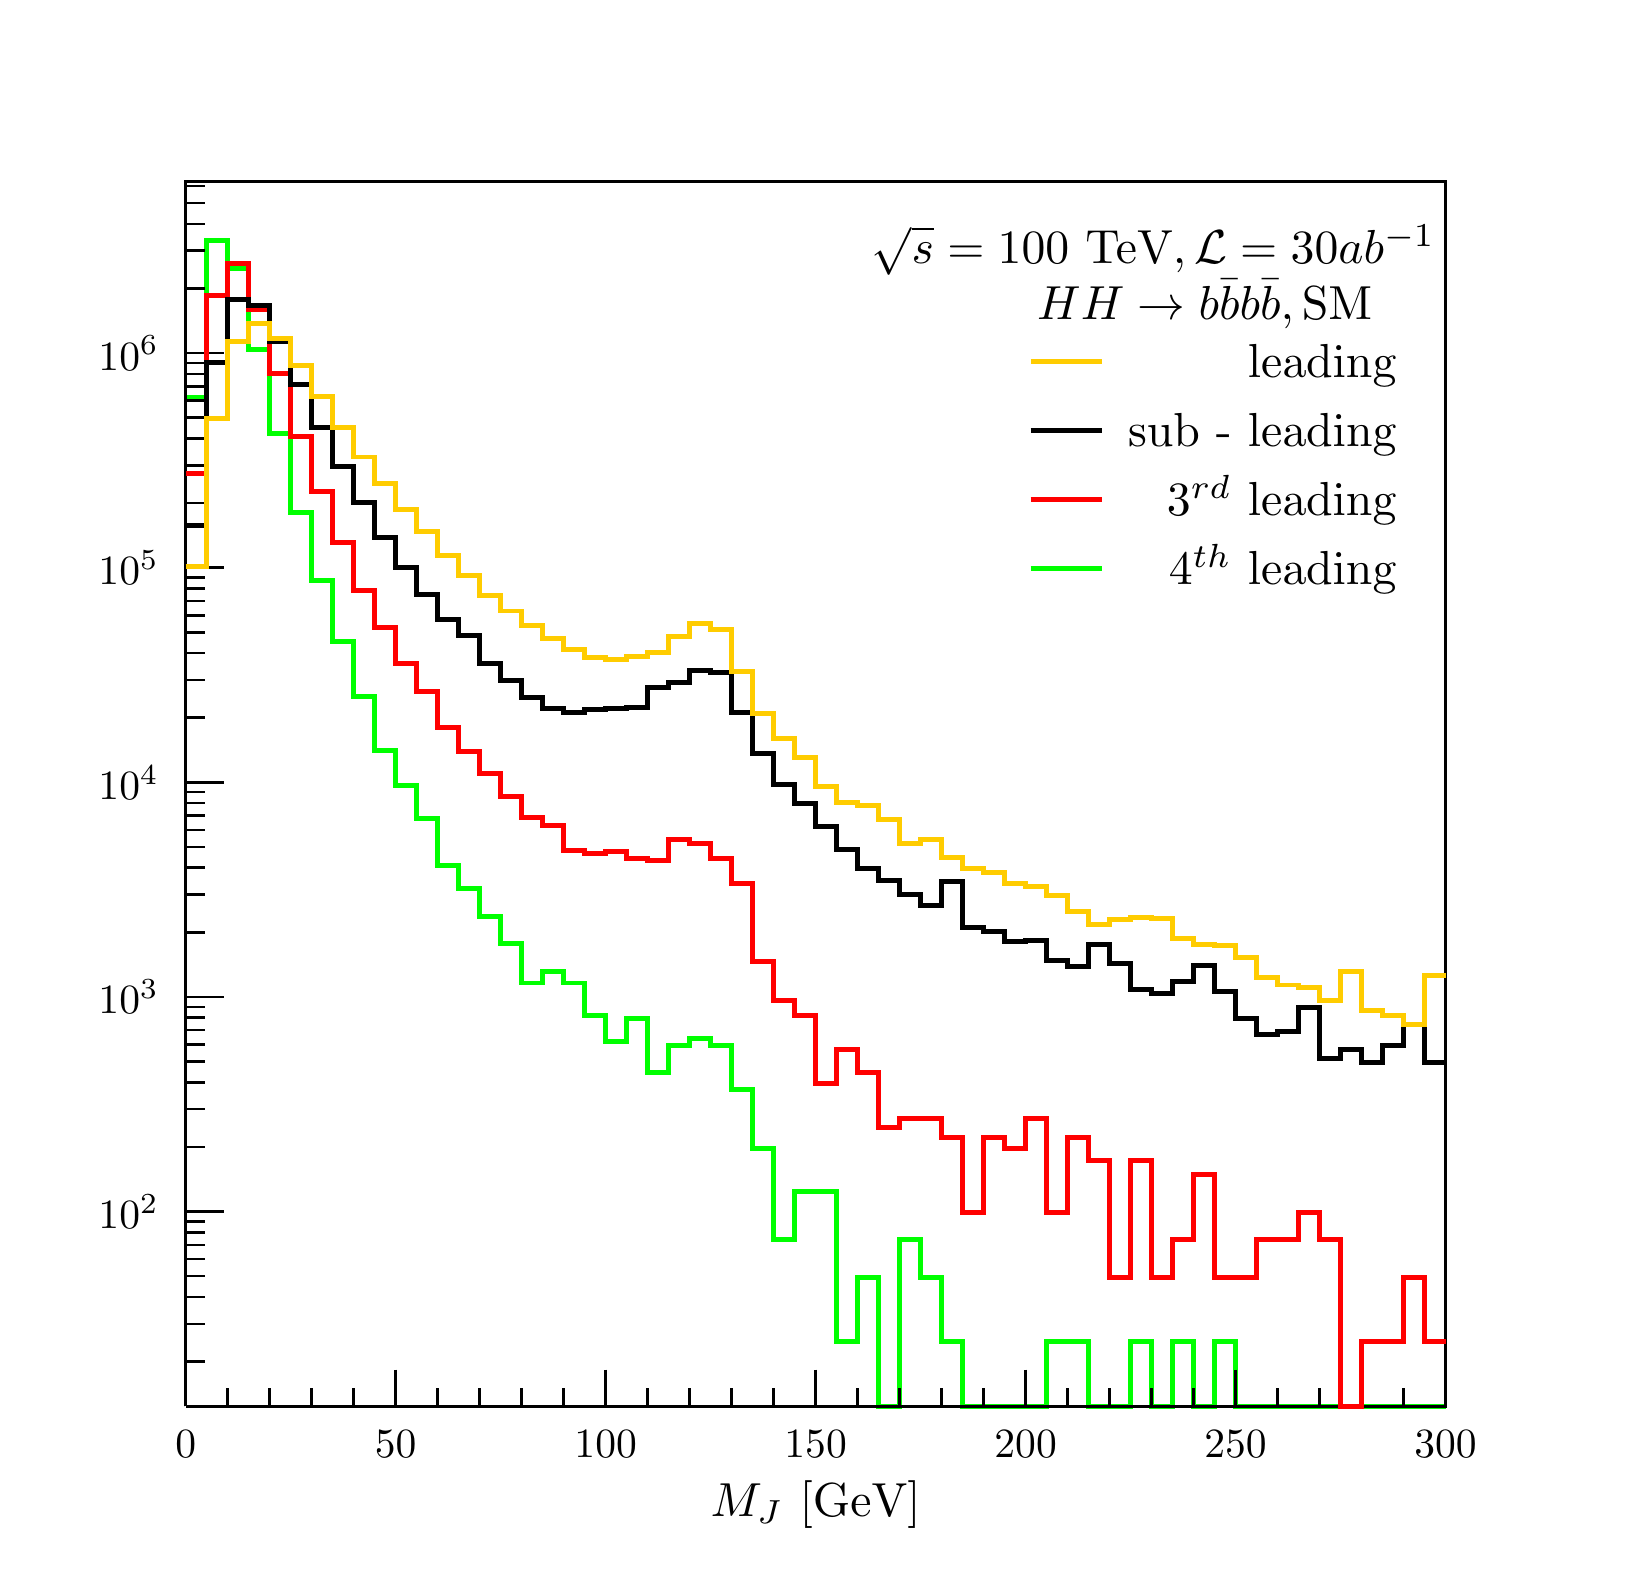
\begin{tikzpicture}
\pgfdeclareplotmark{cross} {
\pgfpathmoveto{\pgfpoint{-0.3\pgfplotmarksize}{\pgfplotmarksize}}
\pgfpathlineto{\pgfpoint{+0.3\pgfplotmarksize}{\pgfplotmarksize}}
\pgfpathlineto{\pgfpoint{+0.3\pgfplotmarksize}{0.3\pgfplotmarksize}}
\pgfpathlineto{\pgfpoint{+1\pgfplotmarksize}{0.3\pgfplotmarksize}}
\pgfpathlineto{\pgfpoint{+1\pgfplotmarksize}{-0.3\pgfplotmarksize}}
\pgfpathlineto{\pgfpoint{+0.3\pgfplotmarksize}{-0.3\pgfplotmarksize}}
\pgfpathlineto{\pgfpoint{+0.3\pgfplotmarksize}{-1.\pgfplotmarksize}}
\pgfpathlineto{\pgfpoint{-0.3\pgfplotmarksize}{-1.\pgfplotmarksize}}
\pgfpathlineto{\pgfpoint{-0.3\pgfplotmarksize}{-0.3\pgfplotmarksize}}
\pgfpathlineto{\pgfpoint{-1.\pgfplotmarksize}{-0.3\pgfplotmarksize}}
\pgfpathlineto{\pgfpoint{-1.\pgfplotmarksize}{0.3\pgfplotmarksize}}
\pgfpathlineto{\pgfpoint{-0.3\pgfplotmarksize}{0.3\pgfplotmarksize}}
\pgfpathclose
\pgfusepathqstroke
}
\pgfdeclareplotmark{cross*} {
\pgfpathmoveto{\pgfpoint{-0.3\pgfplotmarksize}{\pgfplotmarksize}}
\pgfpathlineto{\pgfpoint{+0.3\pgfplotmarksize}{\pgfplotmarksize}}
\pgfpathlineto{\pgfpoint{+0.3\pgfplotmarksize}{0.3\pgfplotmarksize}}
\pgfpathlineto{\pgfpoint{+1\pgfplotmarksize}{0.3\pgfplotmarksize}}
\pgfpathlineto{\pgfpoint{+1\pgfplotmarksize}{-0.3\pgfplotmarksize}}
\pgfpathlineto{\pgfpoint{+0.3\pgfplotmarksize}{-0.3\pgfplotmarksize}}
\pgfpathlineto{\pgfpoint{+0.3\pgfplotmarksize}{-1.\pgfplotmarksize}}
\pgfpathlineto{\pgfpoint{-0.3\pgfplotmarksize}{-1.\pgfplotmarksize}}
\pgfpathlineto{\pgfpoint{-0.3\pgfplotmarksize}{-0.3\pgfplotmarksize}}
\pgfpathlineto{\pgfpoint{-1.\pgfplotmarksize}{-0.3\pgfplotmarksize}}
\pgfpathlineto{\pgfpoint{-1.\pgfplotmarksize}{0.3\pgfplotmarksize}}
\pgfpathlineto{\pgfpoint{-0.3\pgfplotmarksize}{0.3\pgfplotmarksize}}
\pgfpathclose
\pgfusepathqfillstroke
}
\pgfdeclareplotmark{newstar} {
\pgfpathmoveto{\pgfqpoint{0pt}{\pgfplotmarksize}}
\pgfpathlineto{\pgfqpointpolar{44}{0.5\pgfplotmarksize}}
\pgfpathlineto{\pgfqpointpolar{18}{\pgfplotmarksize}}
\pgfpathlineto{\pgfqpointpolar{-20}{0.5\pgfplotmarksize}}
\pgfpathlineto{\pgfqpointpolar{-54}{\pgfplotmarksize}}
\pgfpathlineto{\pgfqpointpolar{-90}{0.5\pgfplotmarksize}}
\pgfpathlineto{\pgfqpointpolar{234}{\pgfplotmarksize}}
\pgfpathlineto{\pgfqpointpolar{198}{0.5\pgfplotmarksize}}
\pgfpathlineto{\pgfqpointpolar{162}{\pgfplotmarksize}}
\pgfpathlineto{\pgfqpointpolar{134}{0.5\pgfplotmarksize}}
\pgfpathclose
\pgfusepathqstroke
}
\pgfdeclareplotmark{newstar*} {
\pgfpathmoveto{\pgfqpoint{0pt}{\pgfplotmarksize}}
\pgfpathlineto{\pgfqpointpolar{44}{0.5\pgfplotmarksize}}
\pgfpathlineto{\pgfqpointpolar{18}{\pgfplotmarksize}}
\pgfpathlineto{\pgfqpointpolar{-20}{0.5\pgfplotmarksize}}
\pgfpathlineto{\pgfqpointpolar{-54}{\pgfplotmarksize}}
\pgfpathlineto{\pgfqpointpolar{-90}{0.5\pgfplotmarksize}}
\pgfpathlineto{\pgfqpointpolar{234}{\pgfplotmarksize}}
\pgfpathlineto{\pgfqpointpolar{198}{0.5\pgfplotmarksize}}
\pgfpathlineto{\pgfqpointpolar{162}{\pgfplotmarksize}}
\pgfpathlineto{\pgfqpointpolar{134}{0.5\pgfplotmarksize}}
\pgfpathclose
\pgfusepathqfillstroke
}
\definecolor{c}{rgb}{1,1,1};
\draw [color=c, fill=c] (0,0) rectangle (20,19.4486);
\draw [color=c, fill=c] (0,0) rectangle (20,19.4486);
\draw [color=c, fill=c] (2,1.94486) rectangle (18,17.5038);
\definecolor{c}{rgb}{0,0,0};
\draw [c,line width=0.9] (2,1.94486) -- (2,17.5038) -- (18,17.5038) -- (18,1.94486) -- (2,1.94486);
\definecolor{c}{rgb}{1,1,1};
\draw [color=c, fill=c] (2,1.94486) rectangle (18,17.5038);
\definecolor{c}{rgb}{0,0,0};
\draw [c,line width=0.9] (2,1.94486) -- (2,17.5038) -- (18,17.5038) -- (18,1.94486) -- (2,1.94486);
\definecolor{c}{rgb}{0,1,0};
\draw [c,line width=1.8] (2,14.7642) -- (2.26667,14.7642) -- (2.26667,16.7473) -- (2.53333,16.7473) -- (2.53333,16.4008) -- (2.8,16.4008) -- (2.8,15.3744) -- (3.06667,15.3744) -- (3.06667,14.2969) -- (3.33333,14.2969) -- (3.33333,13.2996) --
 (3.6,13.2996) -- (3.6,12.4302) -- (3.86667,12.4302) -- (3.86667,11.655) -- (4.13333,11.655) -- (4.13333,10.9552) -- (4.4,10.9552) -- (4.4,10.281) -- (4.66667,10.281) -- (4.66667,9.83067) -- (4.93333,9.83067) -- (4.93333,9.40976) -- (5.2,9.40976) --
 (5.2,8.81655) -- (5.46667,8.81655) -- (5.46667,8.52718) -- (5.73333,8.52718) -- (5.73333,8.16829) -- (6,8.16829) -- (6,7.82776) -- (6.26667,7.82776) -- (6.26667,7.32288) -- (6.53333,7.32288) -- (6.53333,7.4651) -- (6.8,7.4651) -- (6.8,7.32288) --
 (7.06667,7.32288) -- (7.06667,6.90426) -- (7.33333,6.90426) -- (7.33333,6.57562) -- (7.6,6.57562) -- (7.6,6.86784) -- (7.86667,6.86784) -- (7.86667,6.18677) -- (8.13333,6.18677) -- (8.13333,6.5273) -- (8.4,6.5273) -- (8.4,6.62205) --
 (8.66667,6.62205) -- (8.66667,6.5273) -- (8.93333,6.5273) -- (8.93333,5.97095) -- (9.2,5.97095) -- (9.2,5.22685) -- (9.46667,5.22685) -- (9.46667,4.06581) -- (9.73333,4.06581) -- (9.73333,4.67049) -- (10,4.67049) -- (10,4.67049) -- (10.2667,4.67049)
 -- (10.2667,2.76536) -- (10.5333,2.76536) -- (10.5333,3.58585) -- (10.8,3.58585) -- (10.8,1.94486) -- (11.0667,1.94486) -- (11.0667,4.06581) -- (11.3333,4.06581) -- (11.3333,3.58585) -- (11.6,3.58585) -- (11.6,2.76536) -- (11.8667,2.76536) --
 (11.8667,1.94486) -- (12.1333,1.94486) -- (12.1333,1.94486) -- (12.4,1.94486) -- (12.4,1.94486) -- (12.6667,1.94486) -- (12.6667,1.94486) -- (12.9333,1.94486) -- (12.9333,2.76536) -- (13.2,2.76536) -- (13.2,2.76536) -- (13.4667,2.76536) --
 (13.4667,1.94486) -- (13.7333,1.94486) -- (13.7333,1.94486) -- (14,1.94486) -- (14,2.76536) -- (14.2667,2.76536) -- (14.2667,1.94486) -- (14.5333,1.94486) -- (14.5333,2.76536) -- (14.8,2.76536) -- (14.8,1.94486) -- (15.0667,1.94486) --
 (15.0667,2.76536) -- (15.3333,2.76536) -- (15.3333,1.94486) -- (15.6,1.94486) -- (15.6,1.94486) -- (15.8667,1.94486) -- (15.8667,1.94486) -- (16.1333,1.94486) -- (16.1333,1.94486) -- (16.4,1.94486) -- (16.4,1.94486) -- (16.6667,1.94486) --
 (16.6667,1.94486) -- (16.9333,1.94486) -- (16.9333,1.94486) -- (17.2,1.94486) -- (17.2,1.94486) -- (17.4667,1.94486) -- (17.4667,1.94486) -- (17.7333,1.94486) -- (17.7333,1.94486) -- (18,1.94486);
\definecolor{c}{rgb}{0,0,0};
\draw [c,line width=0.9] (2,1.94486) -- (18,1.94486);
\draw [c,line width=0.9] (2,2.41163) -- (2,1.94486);
\draw [c,line width=0.9] (2.53333,2.17825) -- (2.53333,1.94486);
\draw [c,line width=0.9] (3.06667,2.17825) -- (3.06667,1.94486);
\draw [c,line width=0.9] (3.6,2.17825) -- (3.6,1.94486);
\draw [c,line width=0.9] (4.13333,2.17825) -- (4.13333,1.94486);
\draw [c,line width=0.9] (4.66667,2.41163) -- (4.66667,1.94486);
\draw [c,line width=0.9] (5.2,2.17825) -- (5.2,1.94486);
\draw [c,line width=0.9] (5.73333,2.17825) -- (5.73333,1.94486);
\draw [c,line width=0.9] (6.26667,2.17825) -- (6.26667,1.94486);
\draw [c,line width=0.9] (6.8,2.17825) -- (6.8,1.94486);
\draw [c,line width=0.9] (7.33333,2.41163) -- (7.33333,1.94486);
\draw [c,line width=0.9] (7.86667,2.17825) -- (7.86667,1.94486);
\draw [c,line width=0.9] (8.4,2.17825) -- (8.4,1.94486);
\draw [c,line width=0.9] (8.93333,2.17825) -- (8.93333,1.94486);
\draw [c,line width=0.9] (9.46667,2.17825) -- (9.46667,1.94486);
\draw [c,line width=0.9] (10,2.41163) -- (10,1.94486);
\draw [c,line width=0.9] (10.5333,2.17825) -- (10.5333,1.94486);
\draw [c,line width=0.9] (11.0667,2.17825) -- (11.0667,1.94486);
\draw [c,line width=0.9] (11.6,2.17825) -- (11.6,1.94486);
\draw [c,line width=0.9] (12.1333,2.17825) -- (12.1333,1.94486);
\draw [c,line width=0.9] (12.6667,2.41163) -- (12.6667,1.94486);
\draw [c,line width=0.9] (13.2,2.17825) -- (13.2,1.94486);
\draw [c,line width=0.9] (13.7333,2.17825) -- (13.7333,1.94486);
\draw [c,line width=0.9] (14.2667,2.17825) -- (14.2667,1.94486);
\draw [c,line width=0.9] (14.8,2.17825) -- (14.8,1.94486);
\draw [c,line width=0.9] (15.3333,2.41163) -- (15.3333,1.94486);
\draw [c,line width=0.9] (15.8667,2.17825) -- (15.8667,1.94486);
\draw [c,line width=0.9] (16.4,2.17825) -- (16.4,1.94486);
\draw [c,line width=0.9] (16.9333,2.17825) -- (16.9333,1.94486);
\draw [c,line width=0.9] (17.4667,2.17825) -- (17.4667,1.94486);
\draw [c,line width=0.9] (18,2.41163) -- (18,1.94486);
\draw [anchor=base] (2,1.30306) node[scale=1.50291, color=c, rotate=0]{0};
\draw [anchor=base] (4.66667,1.30306) node[scale=1.50291, color=c, rotate=0]{50};
\draw [anchor=base] (7.33333,1.30306) node[scale=1.50291, color=c, rotate=0]{100};
\draw [anchor=base] (10,1.30306) node[scale=1.50291, color=c, rotate=0]{150};
\draw [anchor=base] (12.6667,1.30306) node[scale=1.50291, color=c, rotate=0]{200};
\draw [anchor=base] (15.3333,1.30306) node[scale=1.50291, color=c, rotate=0]{250};
\draw [anchor=base] (18,1.30306) node[scale=1.50291, color=c, rotate=0]{300};
\draw (10,0.700151) node[scale=1.72557, color=c, rotate=0]{$M_{J} ~[\text{GeV}]$};
\draw [c,line width=0.9] (2,1.94486) -- (2,17.5038);
\draw [c,line width=0.9] (2.24,2.51526) -- (2,2.51526);
\draw [c,line width=0.9] (2.24,2.99522) -- (2,2.99522);
\draw [c,line width=0.9] (2.24,3.33575) -- (2,3.33575);
\draw [c,line width=0.9] (2.24,3.59989) -- (2,3.59989);
\draw [c,line width=0.9] (2.24,3.81571) -- (2,3.81571);
\draw [c,line width=0.9] (2.24,3.99818) -- (2,3.99818);
\draw [c,line width=0.9] (2.24,4.15625) -- (2,4.15625);
\draw [c,line width=0.9] (2.24,4.29567) -- (2,4.29567);
\draw [c,line width=0.9] (2.48,4.42039) -- (2,4.42039);
\draw [anchor= east] (1.844,4.42039) node[scale=1.50291, color=c, rotate=0]{$10^{2}$};
\draw [c,line width=0.9] (2.24,5.24089) -- (2,5.24089);
\draw [c,line width=0.9] (2.24,5.72085) -- (2,5.72085);
\draw [c,line width=0.9] (2.24,6.06138) -- (2,6.06138);
\draw [c,line width=0.9] (2.24,6.32552) -- (2,6.32552);
\draw [c,line width=0.9] (2.24,6.54134) -- (2,6.54134);
\draw [c,line width=0.9] (2.24,6.72381) -- (2,6.72381);
\draw [c,line width=0.9] (2.24,6.88188) -- (2,6.88188);
\draw [c,line width=0.9] (2.24,7.0213) -- (2,7.0213);
\draw [c,line width=0.9] (2.48,7.14602) -- (2,7.14602);
\draw [anchor= east] (1.844,7.14602) node[scale=1.50291, color=c, rotate=0]{$10^{3}$};
\draw [c,line width=0.9] (2.24,7.96652) -- (2,7.96652);
\draw [c,line width=0.9] (2.24,8.44648) -- (2,8.44648);
\draw [c,line width=0.9] (2.24,8.78701) -- (2,8.78701);
\draw [c,line width=0.9] (2.24,9.05115) -- (2,9.05115);
\draw [c,line width=0.9] (2.24,9.26697) -- (2,9.26697);
\draw [c,line width=0.9] (2.24,9.44944) -- (2,9.44944);
\draw [c,line width=0.9] (2.24,9.60751) -- (2,9.60751);
\draw [c,line width=0.9] (2.24,9.74693) -- (2,9.74693);
\draw [c,line width=0.9] (2.48,9.87165) -- (2,9.87165);
\draw [anchor= east] (1.844,9.87165) node[scale=1.50291, color=c, rotate=0]{$10^{4}$};
\draw [c,line width=0.9] (2.24,10.6921) -- (2,10.6921);
\draw [c,line width=0.9] (2.24,11.1721) -- (2,11.1721);
\draw [c,line width=0.9] (2.24,11.5126) -- (2,11.5126);
\draw [c,line width=0.9] (2.24,11.7768) -- (2,11.7768);
\draw [c,line width=0.9] (2.24,11.9926) -- (2,11.9926);
\draw [c,line width=0.9] (2.24,12.1751) -- (2,12.1751);
\draw [c,line width=0.9] (2.24,12.3331) -- (2,12.3331);
\draw [c,line width=0.9] (2.24,12.4726) -- (2,12.4726);
\draw [c,line width=0.9] (2.48,12.5973) -- (2,12.5973);
\draw [anchor= east] (1.844,12.5973) node[scale=1.50291, color=c, rotate=0]{$10^{5}$};
\draw [c,line width=0.9] (2.24,13.4178) -- (2,13.4178);
\draw [c,line width=0.9] (2.24,13.8977) -- (2,13.8977);
\draw [c,line width=0.9] (2.24,14.2383) -- (2,14.2383);
\draw [c,line width=0.9] (2.24,14.5024) -- (2,14.5024);
\draw [c,line width=0.9] (2.24,14.7182) -- (2,14.7182);
\draw [c,line width=0.9] (2.24,14.9007) -- (2,14.9007);
\draw [c,line width=0.9] (2.24,15.0588) -- (2,15.0588);
\draw [c,line width=0.9] (2.24,15.1982) -- (2,15.1982);
\draw [c,line width=0.9] (2.48,15.3229) -- (2,15.3229);
\draw [anchor= east] (1.844,15.3229) node[scale=1.50291, color=c, rotate=0]{$10^{6}$};
\draw [c,line width=0.9] (2.24,16.1434) -- (2,16.1434);
\draw [c,line width=0.9] (2.24,16.6234) -- (2,16.6234);
\draw [c,line width=0.9] (2.24,16.9639) -- (2,16.9639);
\draw [c,line width=0.9] (2.24,17.228) -- (2,17.228);
\draw [c,line width=0.9] (2.24,17.4439) -- (2,17.4439);
\definecolor{c}{rgb}{1,0,0};
\draw [c,line width=1.8] (2,13.7935) -- (2.26667,13.7935) -- (2.26667,16.0561) -- (2.53333,16.0561) -- (2.53333,16.4569) -- (2.8,16.4569) -- (2.8,15.8703) -- (3.06667,15.8703) -- (3.06667,15.0662) -- (3.33333,15.0662) -- (3.33333,14.2685) --
 (3.6,14.2685) -- (3.6,13.5587) -- (3.86667,13.5587) -- (3.86667,12.9233) -- (4.13333,12.9233) -- (4.13333,12.3016) -- (4.4,12.3016) -- (4.4,11.8384) -- (4.66667,11.8384) -- (4.66667,11.378) -- (4.93333,11.378) -- (4.93333,11.0223) -- (5.2,11.0223)
 -- (5.2,10.5632) -- (5.46667,10.5632) -- (5.46667,10.258) -- (5.73333,10.258) -- (5.73333,9.97847) -- (6,9.97847) -- (6,9.68935) -- (6.26667,9.68935) -- (6.26667,9.42265) -- (6.53333,9.42265) -- (6.53333,9.32469) -- (6.8,9.32469) -- (6.8,9.00106) --
 (7.06667,9.00106) -- (7.06667,8.96387) -- (7.33333,8.96387) -- (7.33333,8.98879) -- (7.6,8.98879) -- (7.6,8.9058) -- (7.86667,8.9058) -- (7.86667,8.87905) -- (8.13333,8.87905) -- (8.13333,9.14993) -- (8.4,9.14993) -- (8.4,9.10049) --
 (8.66667,9.10049) -- (8.66667,8.9058) -- (8.93333,8.9058) -- (8.93333,8.5806) -- (9.2,8.5806) -- (9.2,7.59204) -- (9.46667,7.59204) -- (9.46667,7.10201) -- (9.73333,7.10201) -- (9.73333,6.90426) -- (10,6.90426) -- (10,6.04734) -- (10.2667,6.04734)
 -- (10.2667,6.47692) -- (10.5333,6.47692) -- (10.5333,6.18677) -- (10.8,6.18677) -- (10.8,5.49099) -- (11.0667,5.49099) -- (11.0667,5.60381) -- (11.3333,5.60381) -- (11.3333,5.60381) -- (11.6,5.60381) -- (11.6,5.36627) -- (11.8667,5.36627) --
 (11.8667,4.40635) -- (12.1333,4.40635) -- (12.1333,5.36627) -- (12.4,5.36627) -- (12.4,5.22685) -- (12.6667,5.22685) -- (12.6667,5.60381) -- (12.9333,5.60381) -- (12.9333,4.40635) -- (13.2,4.40635) -- (13.2,5.36627) -- (13.4667,5.36627) --
 (13.4667,5.06878) -- (13.7333,5.06878) -- (13.7333,3.58585) -- (14,3.58585) -- (14,5.06878) -- (14.2667,5.06878) -- (14.2667,3.58585) -- (14.5333,3.58585) -- (14.5333,4.06581) -- (14.8,4.06581) -- (14.8,4.88631) -- (15.0667,4.88631) --
 (15.0667,3.58585) -- (15.3333,3.58585) -- (15.3333,3.58585) -- (15.6,3.58585) -- (15.6,4.06581) -- (15.8667,4.06581) -- (15.8667,4.06581) -- (16.1333,4.06581) -- (16.1333,4.40635) -- (16.4,4.40635) -- (16.4,4.06581) -- (16.6667,4.06581) --
 (16.6667,1.94486) -- (16.9333,1.94486) -- (16.9333,2.76536) -- (17.2,2.76536) -- (17.2,2.76536) -- (17.4667,2.76536) -- (17.4667,3.58585) -- (17.7333,3.58585) -- (17.7333,2.76536) -- (18,2.76536);
\definecolor{c}{rgb}{0,0,0};
\draw [c,line width=1.8] (2,13.1303) -- (2.26667,13.1303) -- (2.26667,15.2082) -- (2.53333,15.2082) -- (2.53333,16.009) -- (2.8,16.009) -- (2.8,15.9241) -- (3.06667,15.9241) -- (3.06667,15.4694) -- (3.33333,15.4694) -- (3.33333,14.9226) --
 (3.6,14.9226) -- (3.6,14.383) -- (3.86667,14.383) -- (3.86667,13.8806) -- (4.13333,13.8806) -- (4.13333,13.4198) -- (4.4,13.4198) -- (4.4,12.9868) -- (4.66667,12.9868) -- (4.66667,12.6023) -- (4.93333,12.6023) -- (4.93333,12.2521) -- (5.2,12.2521)
 -- (5.2,11.942) -- (5.46667,11.942) -- (5.46667,11.731) -- (5.73333,11.731) -- (5.73333,11.3772) -- (6,11.3772) -- (6,11.165) -- (6.26667,11.165) -- (6.26667,10.9505) -- (6.53333,10.9505) -- (6.53333,10.8123) -- (6.8,10.8123) -- (6.8,10.7596) --
 (7.06667,10.7596) -- (7.06667,10.8016) -- (7.33333,10.8016) -- (7.33333,10.8083) -- (7.6,10.8083) -- (7.6,10.8267) -- (7.86667,10.8267) -- (7.86667,11.0743) -- (8.13333,11.0743) -- (8.13333,11.1452) -- (8.4,11.1452) -- (8.4,11.2913) --
 (8.66667,11.2913) -- (8.66667,11.2637) -- (8.93333,11.2637) -- (8.93333,10.7596) -- (9.2,10.7596) -- (9.2,10.2367) -- (9.46667,10.2367) -- (9.46667,9.84571) -- (9.73333,9.84571) -- (9.73333,9.60084) -- (10,9.60084) -- (10,9.31069) --
 (10.2667,9.31069) -- (10.2667,9.01922) -- (10.5333,9.01922) -- (10.5333,8.77297) -- (10.8,8.77297) -- (10.8,8.62333) -- (11.0667,8.62333) -- (11.0667,8.44226) -- (11.3333,8.44226) -- (11.3333,8.30772) -- (11.6,8.30772) -- (11.6,8.60642) --
 (11.8667,8.60642) -- (11.8667,8.02424) -- (12.1333,8.02424) -- (12.1333,7.98171) -- (12.4,7.98171) -- (12.4,7.84409) -- (12.6667,7.84409) -- (12.6667,7.86019) -- (12.9333,7.86019) -- (12.9333,7.61194) -- (13.2,7.61194) -- (13.2,7.53027) --
 (13.4667,7.53027) -- (13.4667,7.8112) -- (13.7333,7.8112) -- (13.7333,7.57181) -- (14,7.57181) -- (14,7.2448) -- (14.2667,7.2448) -- (14.2667,7.18973) -- (14.5333,7.18973) -- (14.5333,7.3478) -- (14.8,7.3478) -- (14.8,7.55122) -- (15.0667,7.55122)
 -- (15.0667,7.21759) -- (15.3333,7.21759) -- (15.3333,6.86784) -- (15.6,6.86784) -- (15.6,6.66673) -- (15.8667,6.66673) -- (15.8667,6.70977) -- (16.1333,6.70977) -- (16.1333,7.00726) -- (16.4,7.00726) -- (16.4,6.36924) -- (16.6667,6.36924) --
 (16.6667,6.47692) -- (16.9333,6.47692) -- (16.9333,6.31148) -- (17.2,6.31148) -- (17.2,6.5273) -- (17.4667,6.5273) -- (17.4667,6.79144) -- (17.7333,6.79144) -- (17.7333,6.31148) -- (18,6.31148);
\definecolor{c}{rgb}{1,0.8,0};
\draw [c,line width=1.8] (2,12.607) -- (2.26667,12.607) -- (2.26667,14.4871) -- (2.53333,14.4871) -- (2.53333,15.4708) -- (2.8,15.4708) -- (2.8,15.6958) -- (3.06667,15.6958) -- (3.06667,15.5114) -- (3.33333,15.5114) -- (3.33333,15.1654) --
 (3.6,15.1654) -- (3.6,14.772) -- (3.86667,14.772) -- (3.86667,14.3715) -- (4.13333,14.3715) -- (4.13333,14.0029) -- (4.4,14.0029) -- (4.4,13.6606) -- (4.66667,13.6606) -- (4.66667,13.331) -- (4.93333,13.331) -- (4.93333,13.0511) -- (5.2,13.0511) --
 (5.2,12.7556) -- (5.46667,12.7556) -- (5.46667,12.5011) -- (5.73333,12.5011) -- (5.73333,12.2498) -- (6,12.2498) -- (6,12.0471) -- (6.26667,12.0471) -- (6.26667,11.8582) -- (6.53333,11.8582) -- (6.53333,11.6977) -- (6.8,11.6977) -- (6.8,11.5599) --
 (7.06667,11.5599) -- (7.06667,11.4526) -- (7.33333,11.4526) -- (7.33333,11.4285) -- (7.6,11.4285) -- (7.6,11.4701) -- (7.86667,11.4701) -- (7.86667,11.5228) -- (8.13333,11.5228) -- (8.13333,11.7206) -- (8.4,11.7206) -- (8.4,11.8889) --
 (8.66667,11.8889) -- (8.66667,11.8126) -- (8.93333,11.8126) -- (8.93333,11.2763) -- (9.2,11.2763) -- (9.2,10.7457) -- (9.46667,10.7457) -- (9.46667,10.4323) -- (9.73333,10.4323) -- (9.73333,10.1862) -- (10,10.1862) -- (10,9.8246) -- (10.2667,9.8246)
 -- (10.2667,9.61908) -- (10.5333,9.61908) -- (10.5333,9.57858) -- (10.8,9.57858) -- (10.8,9.40109) -- (11.0667,9.40109) -- (11.0667,9.09487) -- (11.3333,9.09487) -- (11.3333,9.13912) -- (11.6,9.13912) -- (11.6,8.9124) -- (11.8667,8.9124) --
 (11.8667,8.77297) -- (12.1333,8.77297) -- (12.1333,8.72002) -- (12.4,8.72002) -- (12.4,8.58927) -- (12.6667,8.58927) -- (12.6667,8.54526) -- (12.9333,8.54526) -- (12.9333,8.43244) -- (13.2,8.43244) -- (13.2,8.2284) -- (13.4667,8.2284) --
 (13.4667,8.0653) -- (13.7333,8.0653) -- (13.7333,8.13071) -- (14,8.13071) -- (14,8.1559) -- (14.2667,8.1559) -- (14.2667,8.14337) -- (14.5333,8.14337) -- (14.5333,7.89176) -- (14.8,7.89176) -- (14.8,7.8112) -- (15.0667,7.8112) -- (15.0667,7.79441)
 -- (15.3333,7.79441) -- (15.3333,7.65075) -- (15.6,7.65075) -- (15.6,7.39612) -- (15.8667,7.39612) -- (15.8667,7.29742) -- (16.1333,7.29742) -- (16.1333,7.2714) -- (16.4,7.2714) -- (16.4,7.10201) -- (16.6667,7.10201) -- (16.6667,7.4651) --
 (16.9333,7.4651) -- (16.9333,6.97392) -- (17.2,6.97392) -- (17.2,6.90426) -- (17.4667,6.90426) -- (17.4667,6.79144) -- (17.7333,6.79144) -- (17.7333,7.41956) -- (18,7.41956);
\definecolor{c}{rgb}{0,0,0};
\draw [anchor=base east] (17.5904,15.0107) node[scale=1.72655, color=c, rotate=0]{~\text{leading}};
\definecolor{c}{rgb}{1,0.8,0};
\draw [c,line width=1.8] (12.7304,15.2185) -- (13.6376,15.2185);
\definecolor{c}{rgb}{0,0,0};
\draw [anchor=base east] (17.5904,14.1355) node[scale=1.72655, color=c, rotate=0]{\text{sub}~-~\text{leading}};
\draw [c,line width=1.8] (12.7304,14.3434) -- (13.6376,14.3434);
\draw [anchor=base east] (17.5904,13.2603) node[scale=1.72655, color=c, rotate=0]{$3^{rd} ~\text{leading}$};
\definecolor{c}{rgb}{1,0,0};
\draw [c,line width=1.8] (12.7304,13.4682) -- (13.6376,13.4682);
\definecolor{c}{rgb}{0,0,0};
\draw [anchor=base east] (17.5904,12.3851) node[scale=1.72655, color=c, rotate=0]{$4^{th} ~\text{leading}$};
\definecolor{c}{rgb}{0,1,0};
\draw [c,line width=1.8] (12.7304,12.593) -- (13.6376,12.593);
\definecolor{c}{rgb}{0,0,0};
\draw [anchor= west] (10.5,16.6286) node[scale=1.72557, color=c, rotate=0]{$\sqrt{s} = 100 ~\text{TeV}, \mathcal{L} = 30 ab^{-1}$};
\draw [anchor= west] (12.6,15.9479) node[scale=1.72557, color=c, rotate=0]{$HH \rightarrow b\bar{b}b\bar{b},\text{SM}$};
\end{tikzpicture}
% end document
\end{document}
